\chapter{Results}\label{chap:res}

\section{Contiguous fill method results}

\begin{figure}
\label{fig:fuse}
\begin{center}
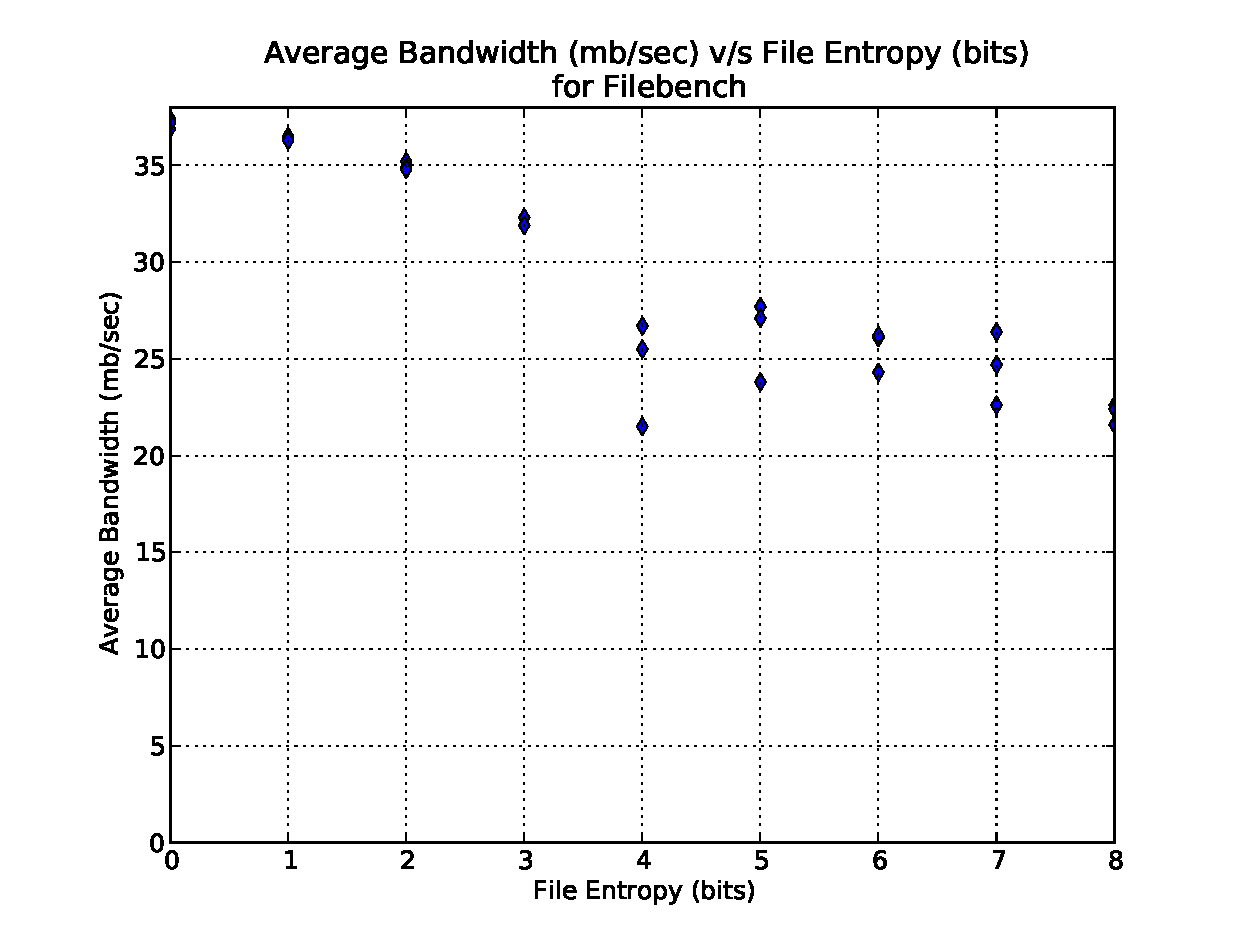
\includegraphics[scale=.55]{../results/write_bw_all.eps}
\caption{Userspace file system architecture in linux\cite{web:wiki-fuse}}
\end{center}
\end{figure}

\begin{figure}
\label{fig:fuse}
\begin{center}
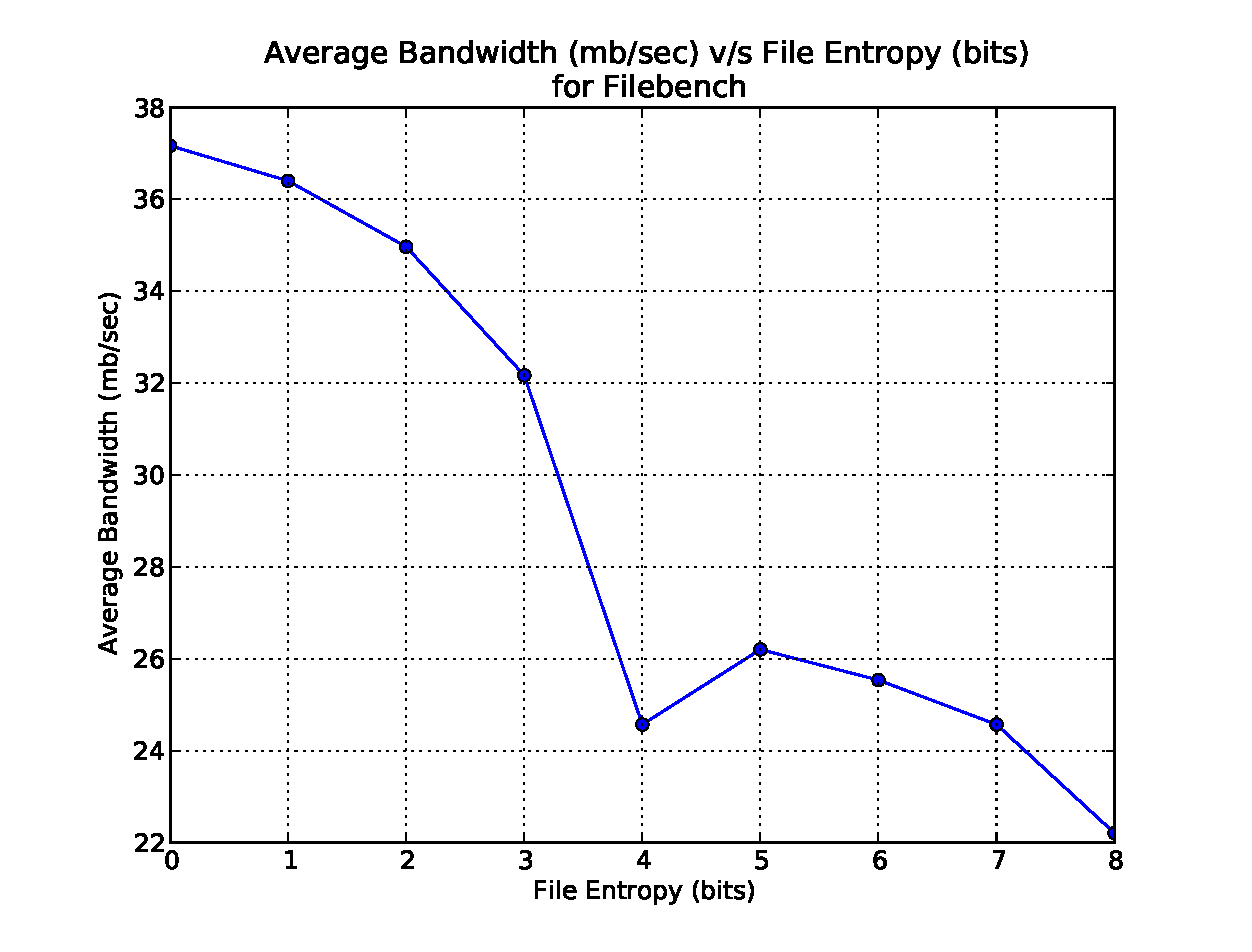
\includegraphics[scale=.55]{../results/write_bw_avg.eps}
\caption{Userspace file system architecture in linux\cite{web:wiki-fuse}}
\end{center}
\end{figure}


\begin{figure}
\label{fig:fuse}
\begin{center}
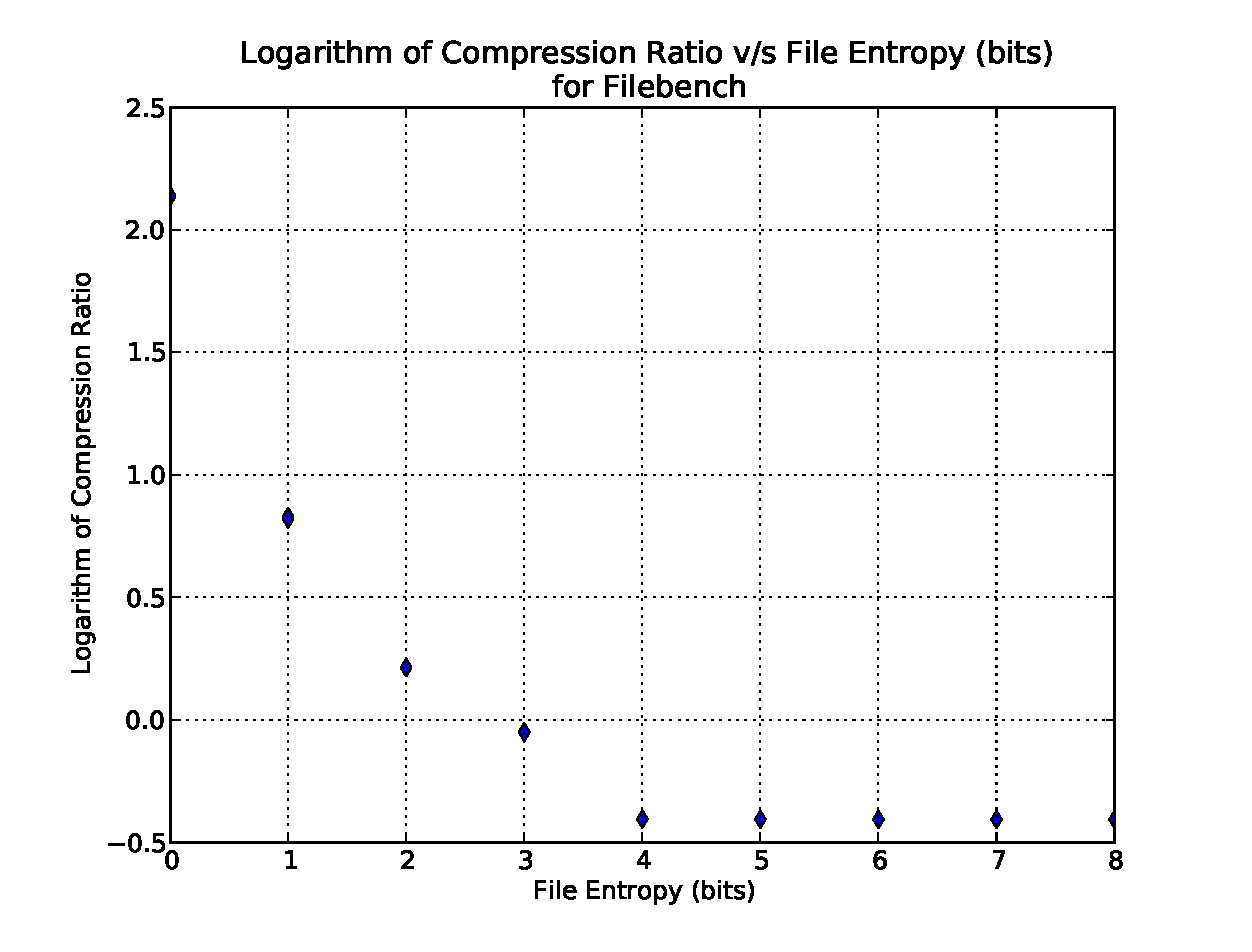
\includegraphics[scale=.55]{../results/write_comp_all.eps}
\caption{Userspace file system architecture in linux\cite{web:wiki-fuse}}
\end{center}
\end{figure}


\begin{figure}
\label{fig:fuse}
\begin{center}
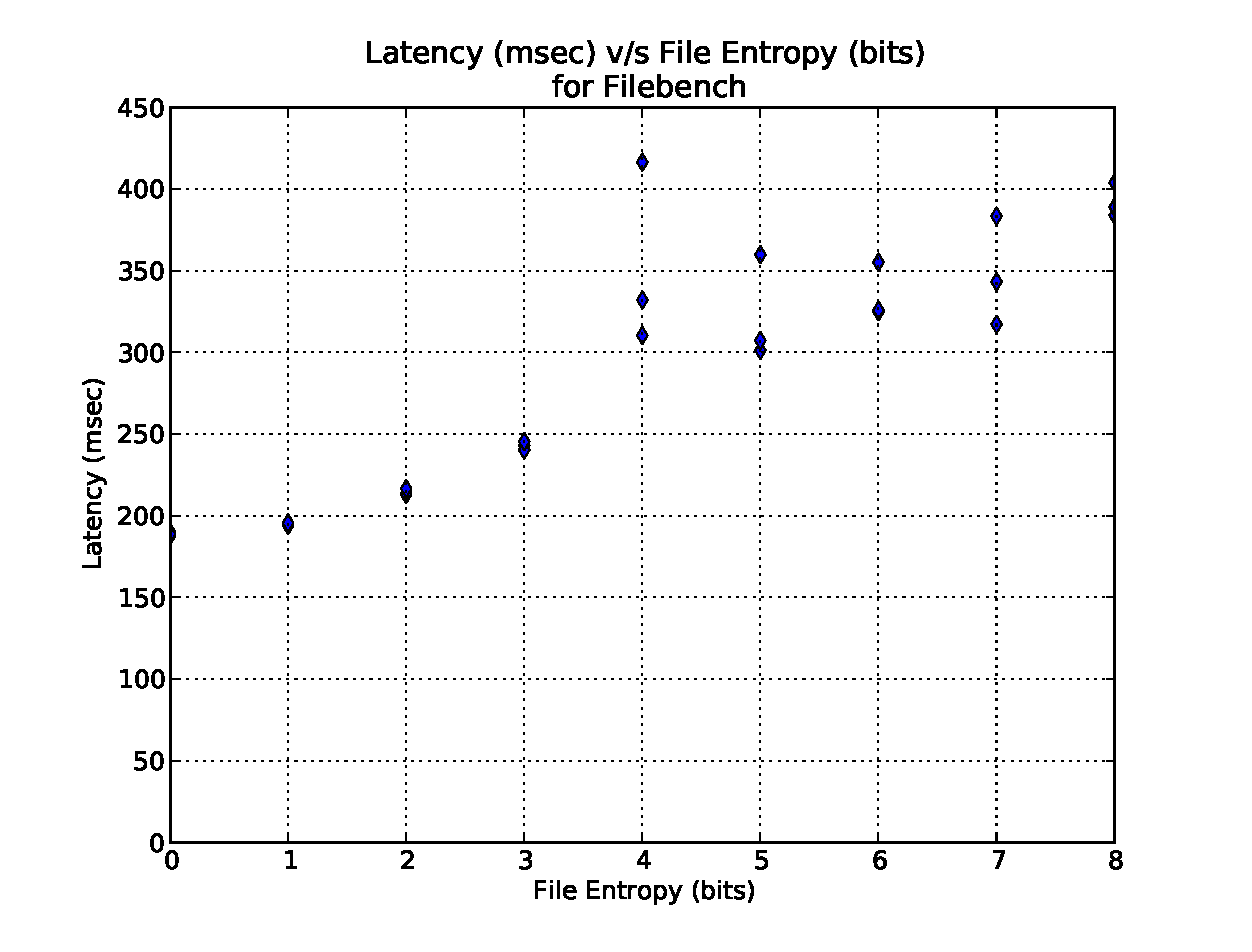
\includegraphics[scale=.55]{../results/write_latency_all.eps}
\caption{Userspace file system architecture in linux\cite{web:wiki-fuse}}
\end{center}
\end{figure}


\begin{figure}
\label{fig:fuse}
\begin{center}
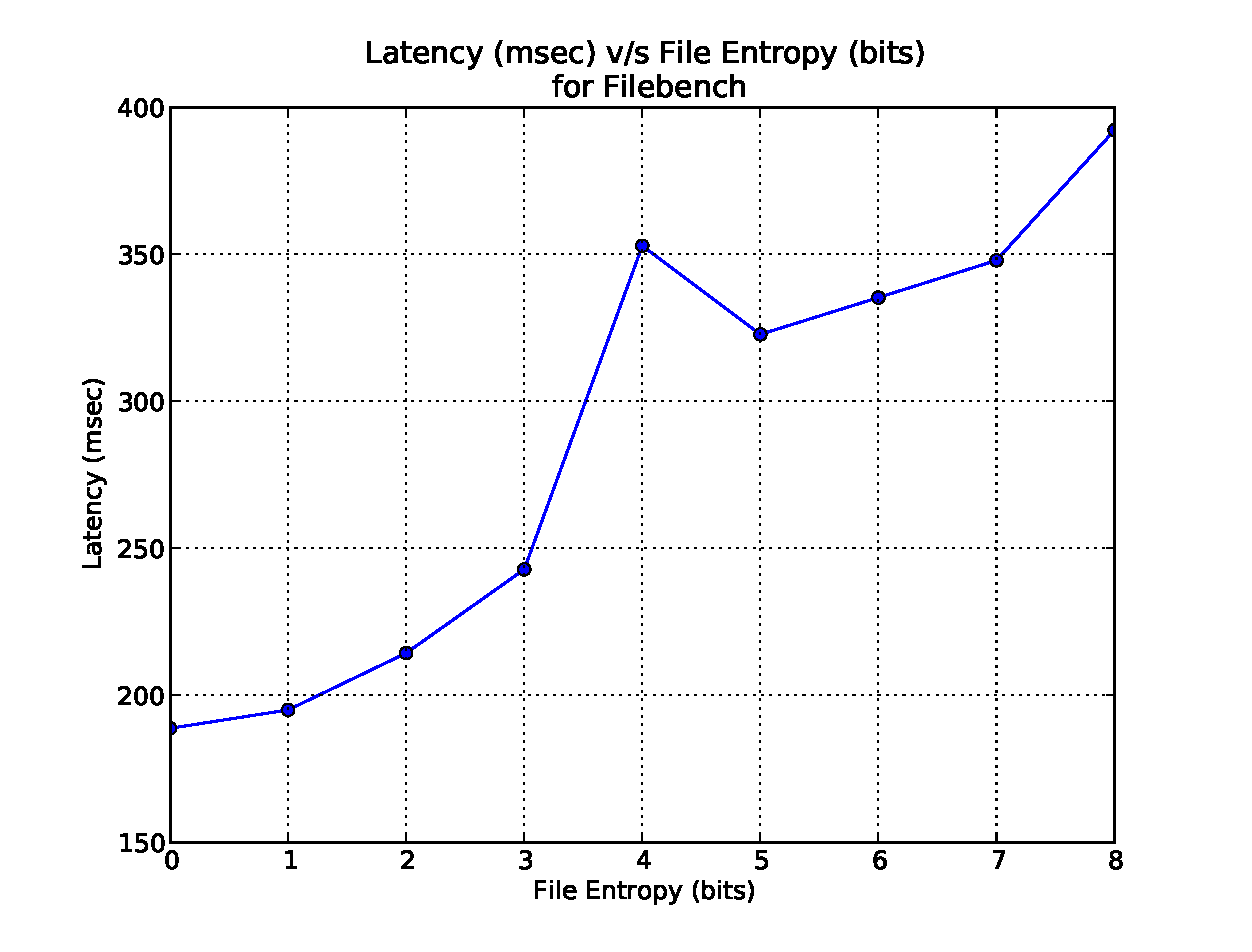
\includegraphics[scale=.55]{../results/write_latency_avg.eps}
\caption{Userspace file system architecture in linux\cite{web:wiki-fuse}}
\end{center}
\end{figure}

\begin{figure}
\label{fig:fuse}
\begin{center}
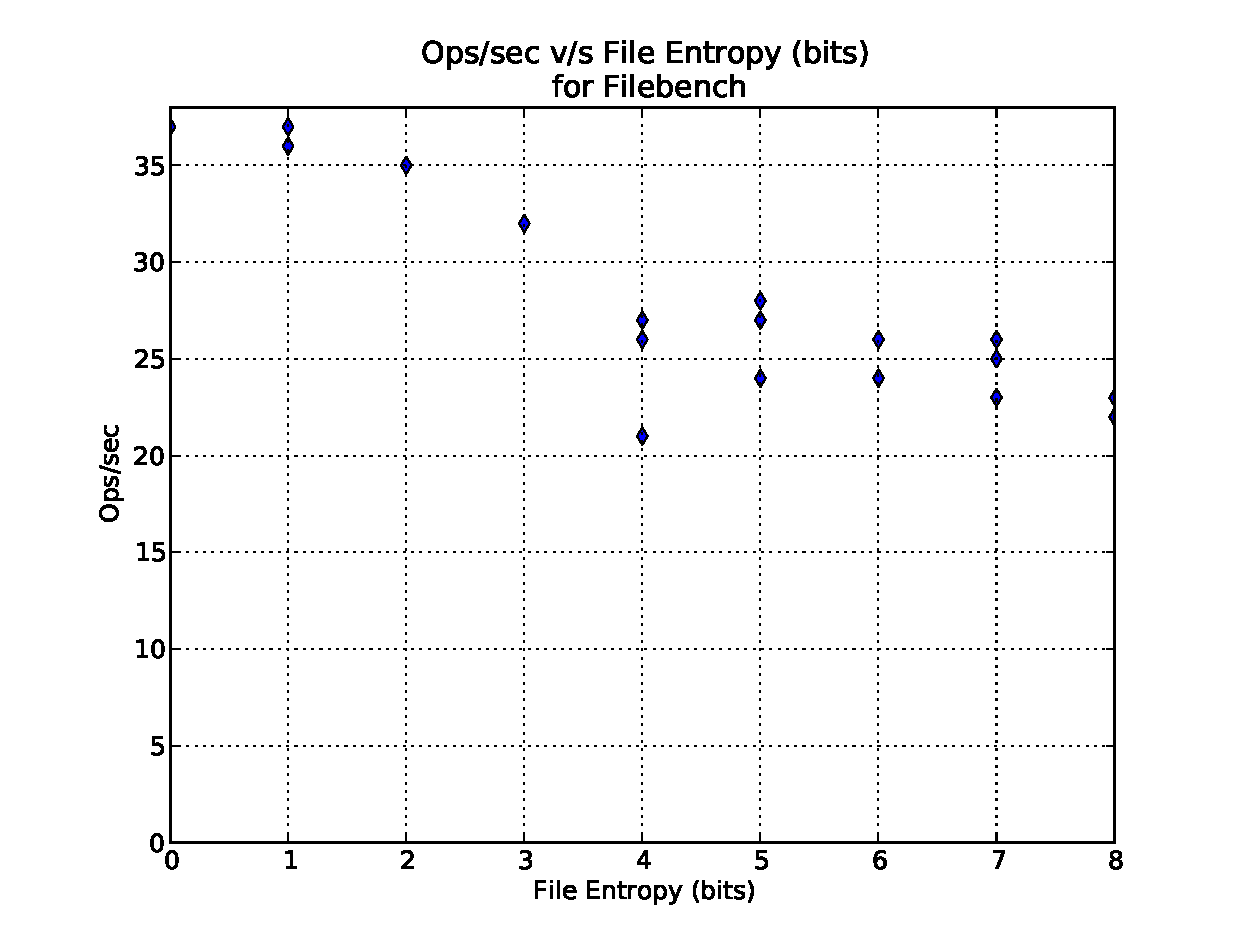
\includegraphics[scale=.55]{../results/write_ops_all.eps}
\caption{Userspace file system architecture in linux\cite{web:wiki-fuse}}
\end{center}
\end{figure}


\begin{figure}
\label{fig:fuse}
\begin{center}
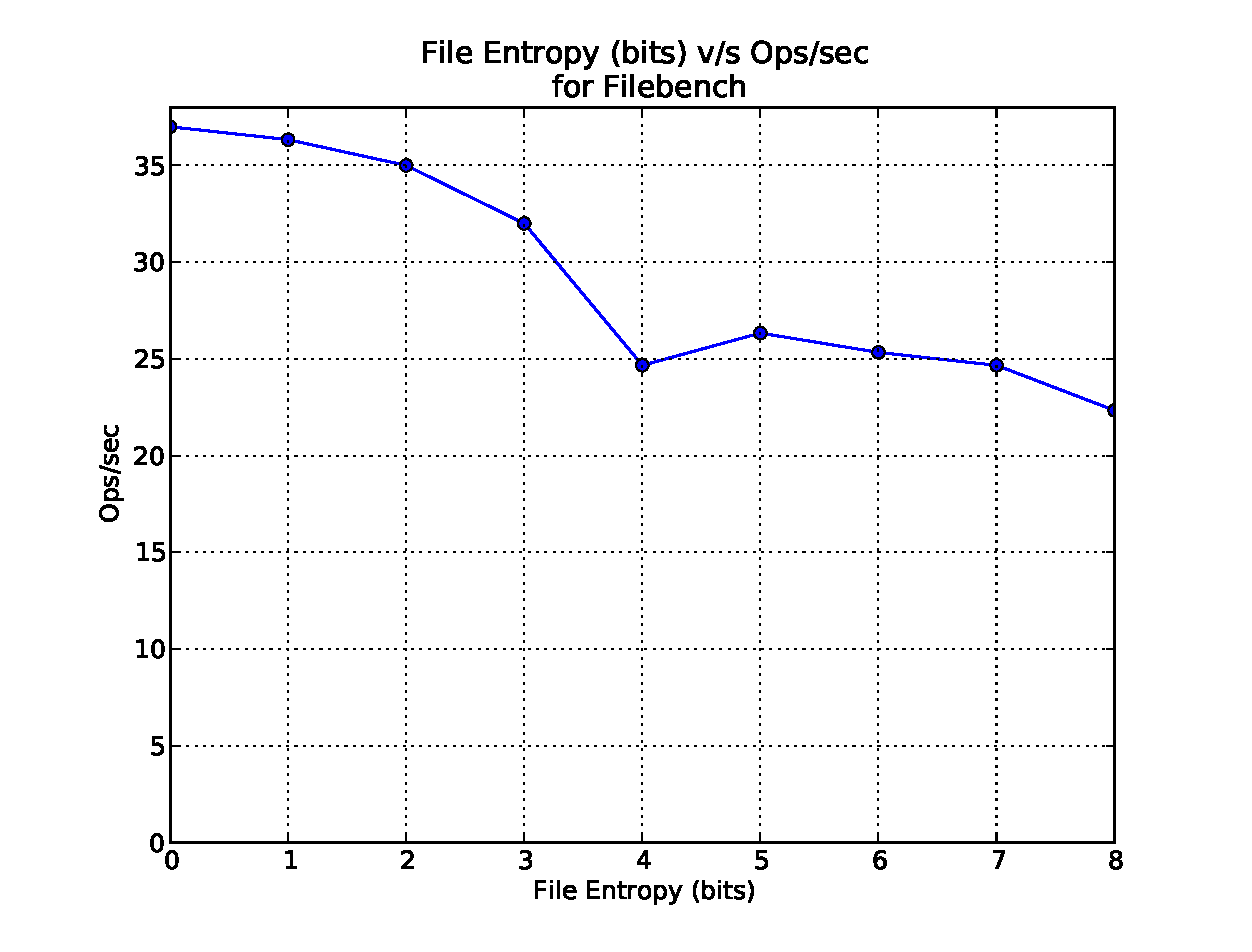
\includegraphics[scale=.55]{../results/write_ops_avg.eps}
\caption{Userspace file system architecture in linux\cite{web:wiki-fuse}}
\end{center}
\end{figure}

\begin{figure}
\label{fig:fuse}
\begin{center}
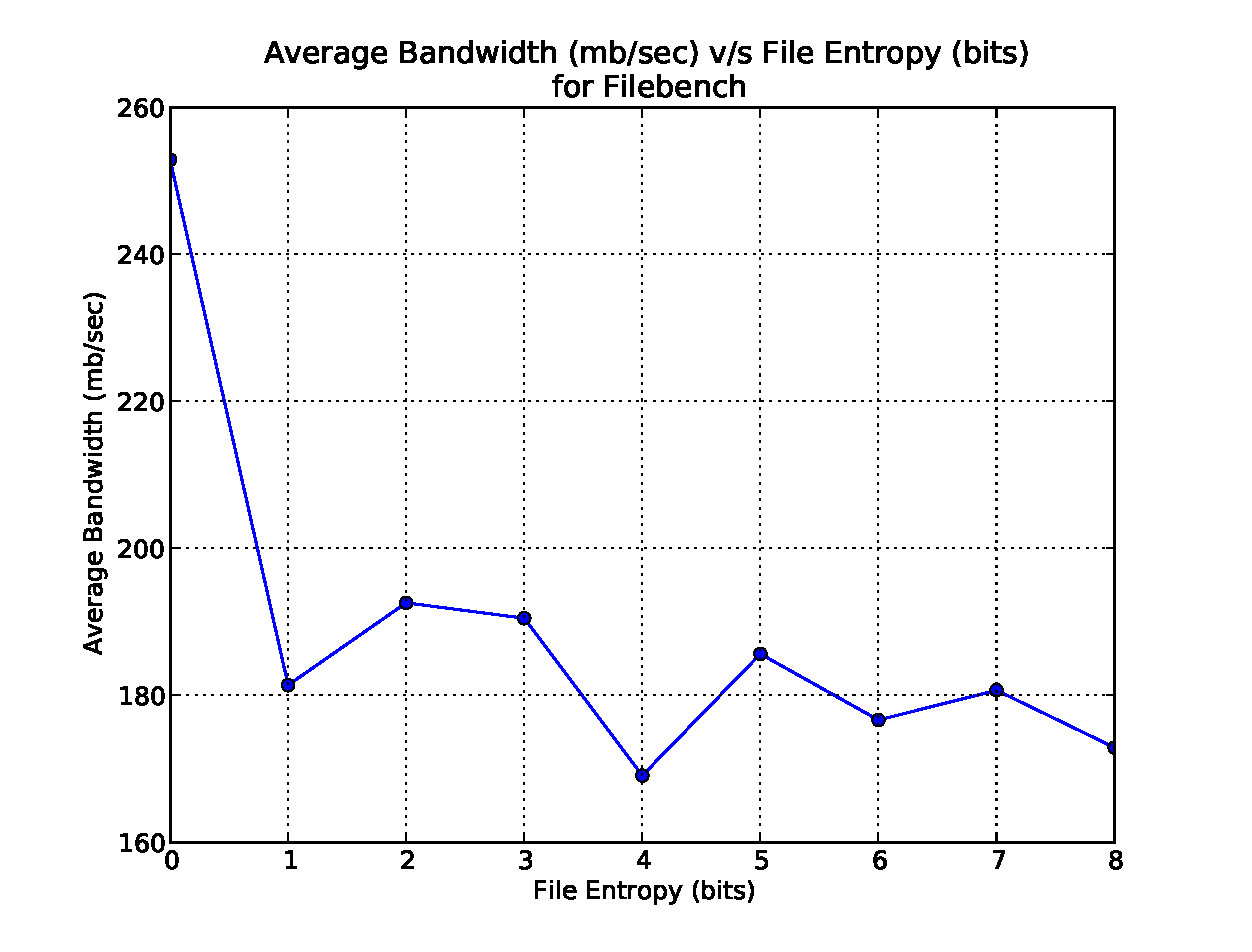
\includegraphics{../results/read_bw.eps}
\caption{Userspace file system architecture in linux\cite{web:wiki-fuse}}
\end{center}
\end{figure}

\begin{figure}
\label{fig:fuse}
\begin{center}
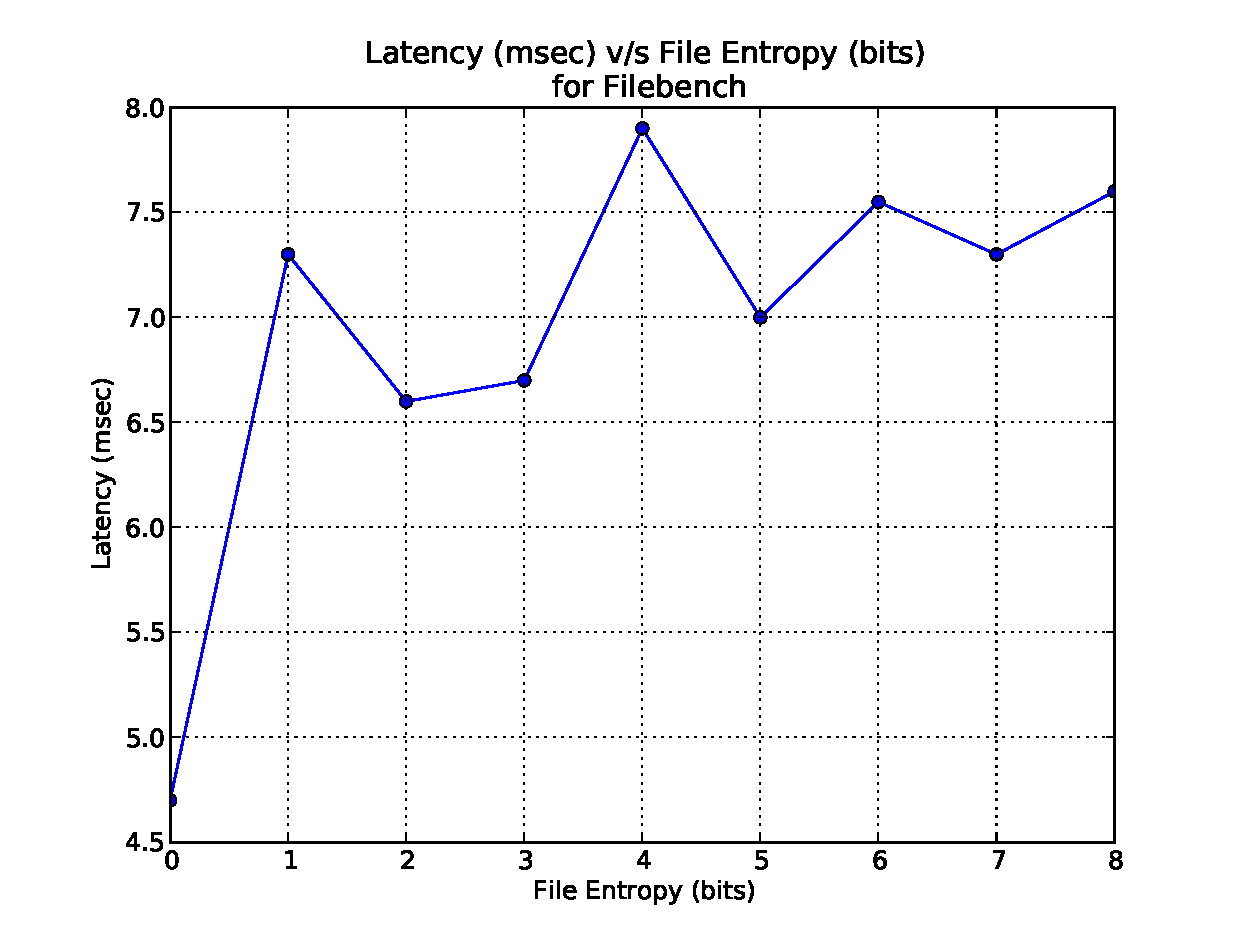
\includegraphics[scale=.55]{../results/read_latency.eps}
\caption{Userspace file system architecture in linux\cite{web:wiki-fuse}}
\end{center}
\end{figure}


\section{Lookup fill method results}


\chapter{Conclusions}\label{chap:conc}
\chapter{Future Work}\label{chap:fut}


Currently generating the random data takes a lot of time, except for the contiguous method explained in section \ref{sec:ent_imp}.
This makes the processor lags behind the disk, which keeps the disk idle most of the time.
 However, this should not affect the results when we compare the readings obtained from different levels of an entropy used with a deduplication file system.
 However, testing other non-deduplication filesystems with entropy generation enabled will cause unexpected results because of the way the statistics are collected in Filebench.
\paragraph{}
 Filebench calculates the averages bandwidth and operations per second.
 Therefore, if the entropy is enabled while running filebench on ext2 for example, most of the time the disk will be idle which will result in lower readings than the case if entropy is switched off, although ext2 is not aware of the data that is being written the previous scenario 
\paragraph{}
To fix this, Filebench has to be modified to calculate the time the disk is actually used and use only that time to calculate the average bandwidth and operations per second.
\paragraph{}
Another point to mention is the model we are using to model practical loads. We are using entropy as the only characteristics of the file that is actually varied.
 Moreover, it is the same value across all the files. In normal loads like the ones in cloud computing servers where there is a lot of backups and snapshots, the entropy can high per file but the redundancy is also high.
 Using true randomization makes it so hard to generate any chunk of the file twice.
 Maybe it is better to generate a more realistic model by profiling large amount of storage and construct the PDF from that data. We can use such PDF to to calculate the probability that a page will be redundant to one already have been written on the disk.
